\chapter{Implementierung}
\label{ch:Implementierung}

In diesem Kapitel wird erläutert, wie die Daten des Datensatzes gesammelt, zur weiteren Verarbeitung vorbereitet und schließlich analysiert werden.
Der Fokus hierbei liegt auf der Implementierung, für mehr Details, siehe Kapitel \todo{link to ref} %verlinke auf kapitel, wo erklärt wird, was wie gemacht wird

\section{App}
\label{ch:Implementierung:app}
\subsection{Plattform}
\label{ch:Implementierung:app:platform}
Die Smartphone-App wurde mit der Sprache Swift für Apple-Smartphones entwickelt. 
Mit der Software XCode lässt sich eine mit Swift geschriebe App kompilieren und auf dem Smartphone installieren.

Zur Einbindung externer Frameworks wird der Dependency-Manager \textit{Accio} und \textit{Carthage} verwendet.
Im Folgenden sind die relevanten Frameworks aufgelistet, welche in der App eingebunden worden sind:

\begin{center}
  \begin{tabular}{ | l | l | }
    \hline
    Imperio & Strukturierung der App \\ \hline
    Realm-Cocoa & Datenbank-Framework \\ \hline
    Zip & Bietet die Möglichkeit, einen Ordner \\ 
    & als {\glqq zip\grqq}-Datei zu komprimieren\\ \hline
    Mungohealer & Fügt Logging zu der App hinzu \\
    \hline
  \end{tabular}
\end{center}

Durch das Framework \textit{Imperio} ist es möglich, die View-Komponenten von der Logik zu trennen. 
Somit ändert sich die Struktur der App, indem jeder Ablauf in der App als \textit{Flow} interpretiert wird. 
Pro Flow wird ein \textit{FlowController} angelegt, welcher die Logik des Ablaufs kontrolliert. 
Ein Flow kann nun beliebig viele \textit{ViewController} starten.
Jede \textit{View}, welche von einem Flow aufgerufen wird, hält ein \textit{Delegate} Objekt.
Ein \textit{Delegate} ist ein Protocol, womit dem \textit{Flow} eine Aktion auf der \textit{View} mitgeteilt werden kann.
Somit wird bei jeder Aktion auf der View eine Funktion des FlowControllers aufgerufen, welcher die View gestartet hat.


Das Framework \textit{Realm} ist eine Datenbank für mobile Systeme, die vollständig auf dem mobilen Endgerät läuft.
Die Daten können direkt als \textit{Objekt} ausgelesen und verarbeitet werden.
In der App wird die Datenbank verwendet, um eine Messung abzuspeichern (siehe Abbildung \ref{implementation:app:erModel}))

Die App ist in 3 Sektionen aufgeteilt, einer \textit{Chartansicht}, einer \textit{Messungsansicht}, sowie einer \textit{Einstellungsansicht}. 
(Abb. \ref{implementation:app:screenshots} Tabbar)
Im weiteren wird nur die \textit{Messungsansicht} genauer erläutert, da die anderen Ansichten im Rahmen der Bachelorarbeit nicht relevant sind.

\begin{figure}[ht]
  \centering
  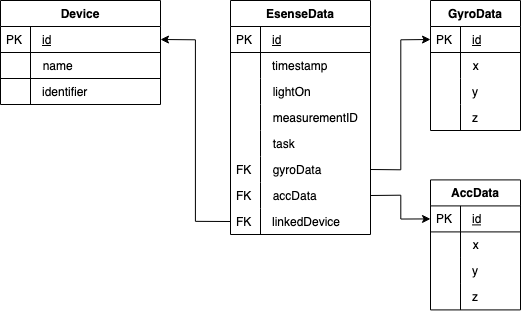
\includegraphics[width=0.7\textwidth]{implementation/app/Database_SleepEar}
  \caption{ER-Diagramm der App-Datenbank\todo{higher resolution}}
  \label{implementation:app:erModel}
\end{figure}

\subsection{Messungsablauf}
\label{ch:Implementierung:app:measurement_procedure}
Mit der Messungsansicht soll eine komplette Messung durchgeführt werden.
Der \textit{MeasurementFlow} wird gestartet und die erste \textit{View} (Abb. \ref{implementation:app:screenshots:connect_bluetooth}) wird geöffnet.
Nach der erfolgreichen Verbindung mit den eSense-Earpods erfolgt eine Weiterleitung zur nächsten \textit{View} (Abb. \ref{implementation:app:screenshots:user_studies_information}) zum Ausfüllen der Nutzerinformationen. 
Mit dem Betätigen des Buttons: {\glqq Start Measurement\grqq} bestätigt man die Eingabe der Daten und die Messung beginnt.
Automatisch beginnt der erste Timer (Abb. \ref{implementation:app:screenshots:measurement_started}).
Der Timer zeigt den aktuellen, sowie den nächsten \textit{Task} an, sowie die Restzeit des aktuellen Tasks.
Der genaue Ablauf der einzelnen Timer ist in Abbildung \ref{fig_study_flow} detailliert beschrieben.
Nach dem Ablauf des letzten Timers wird eine View geöffnet, welche die Möglichkeit zum Teilen der aktuellen Messung bietet (Abb. \ref{implementation:app:screenshots:sampling_stopped}, \ref{implementation:app:screenshots:share}).
Zudem kann die Datenbank vollständig geleert werden.

\subsection{Messung}
\label{ch:Implementierung:app:measurement}
Eine Messung wird im Code in einem \textit{Measurement} Objekt persistiert.
Durch ein Observer-Pattern wird der \textit{MeasurementFlow} über jegliche Änderung informiert und kann entsprechende Handlungen durchführen.
Durch die Funktionen \texttt{startMeasurement} und \texttt{stopMeasurement} kann eine Messung gestartet, bzw gestoppt werden.
Mit der Funktion \texttt{startMeasurement} wird das IMU-Sampling per BLE, sowie die Audioaufnahme gestartet. 
Ebenso wird der erste Timer gestartet und ein doppeltes Lichtsignal gesendet. 
Durch die Funktion \texttt{stopMeasurement} werden die Datenströme gestoppt, ebenfalls ein doppeltes Lichtsignal gesendet und der Timer wird beendet.
Der nächste Task wird gestartet, wenn der Timer abgelaufen ist. Der Timer startet mit der Länge des nächsten Tasks.
Sofern der nächste Task {\glqq Hold\_breath\grqq} ist, also die Person im folgenden Task die Luft anhält, wird dem Teilnehmer kurz vor Ablauf mitgeteilt, wann der nächste Task startet.
Mit der Instruktion \glqq Bitte die Luft anhalten in 3, 2, 1\grqq \ weiß der Teilnehmer, wann er die Luft anhalten soll.
Durch die Anweisung \glqq Stopp\grqq \ wird dem Nutzer das Ende des Tasks mitgeteilt. 
Die Instruktionen liegen als Audiodatei vor und werden jeweils vor dem jeweiligen Task abgespielt und mittels Bluetooth über die Lautsprecher der eSense-Earpods ausgegeben.

\todo{extend with diagrams like class-diagram}

\section{Anbindung an Auswertungspipeline}
\label{ch:Implementierung:way_to_pipeline}
\begin{wrapfigure}{r}{0.3\textwidth}
  \centering
  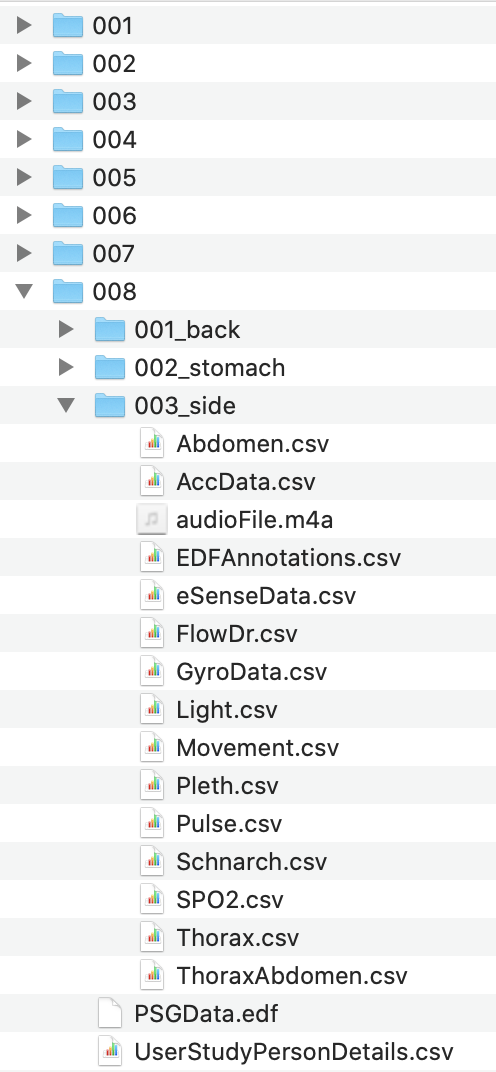
\includegraphics[width=0.25\textwidth]{data_analyzation/folder_structure}
  \caption{Ornderstruktur des Datensatzes}
  \label{implementation:folder_structure}
\end{wrapfigure}
Die App liefert beim Export die Daten der eSense-Earpods, was die IMU-Daten, sowie die Nutzerinformationen und die Mikrofonaufnahme beinhaltet.
Zum aktuellen Stand liegen somit die Daten der eSense-Earpods und vom PSG-System vor. 
Zu Beginn müssen die PSG-Daten, welche als eine Messung für alle 3 Positionen pro Studienteilnehmer persistiert wurde, in 3 einzelne Messungen aufgeteilt werden.
Die Daten des PSG-Systems liegen als \textit{edf}-Datei vor. 
Diese können mittels python und der Library \texttt{edfrd} ausgelesen werden.
Jedoch sind die Einträge des jeweiligen Signals ohne einen Zeitwert abgespeichert. 
Es muss nun aufgrund der Abtastrate in $\si{\hertz}$ die Zeit manuell berechnet werden. 
Mittels der Funktion \texttt{find\_peaks} aus \texttt{scipy.peak}\ können die Peaks des Lichtsensors am PSG-System ermittelt werden (siehe Abb. \ref{implementation:synchronisation:light_peaks_detection}).
Da eine Messung mit 2 Lichtblitzen beginnt und endet, kann nun der Start- und Endzeitpunkt einer Position ermittelt und die einzelnen Positionen können voneinander unterschieden werden. 
Daraufhin können die 11 verfügbaren Signale einzeln ausgelesen werden.
Pro Position wird nun jedes der Signale als \textit{csv}-Datei im jeweiligen Ordner abgelegt.
Die Daten der eSense-Earpods liegen getrennt in \textit{AccData\_\$ID\$.csv} und \textit{GyroData\_\$ID\$.csv} vor. 
Diese werden ausgelesen und zu der Datei \textit{eSenseData.csv} zusammengeführt.
Die Ornderstruktur kann der Abb. \ref{implementation:folder_structure} entnommen werden und ist nun vollständig.

\begin{figure}[ht]
  \centering
  \begin{subfigure}{.25\textwidth}
    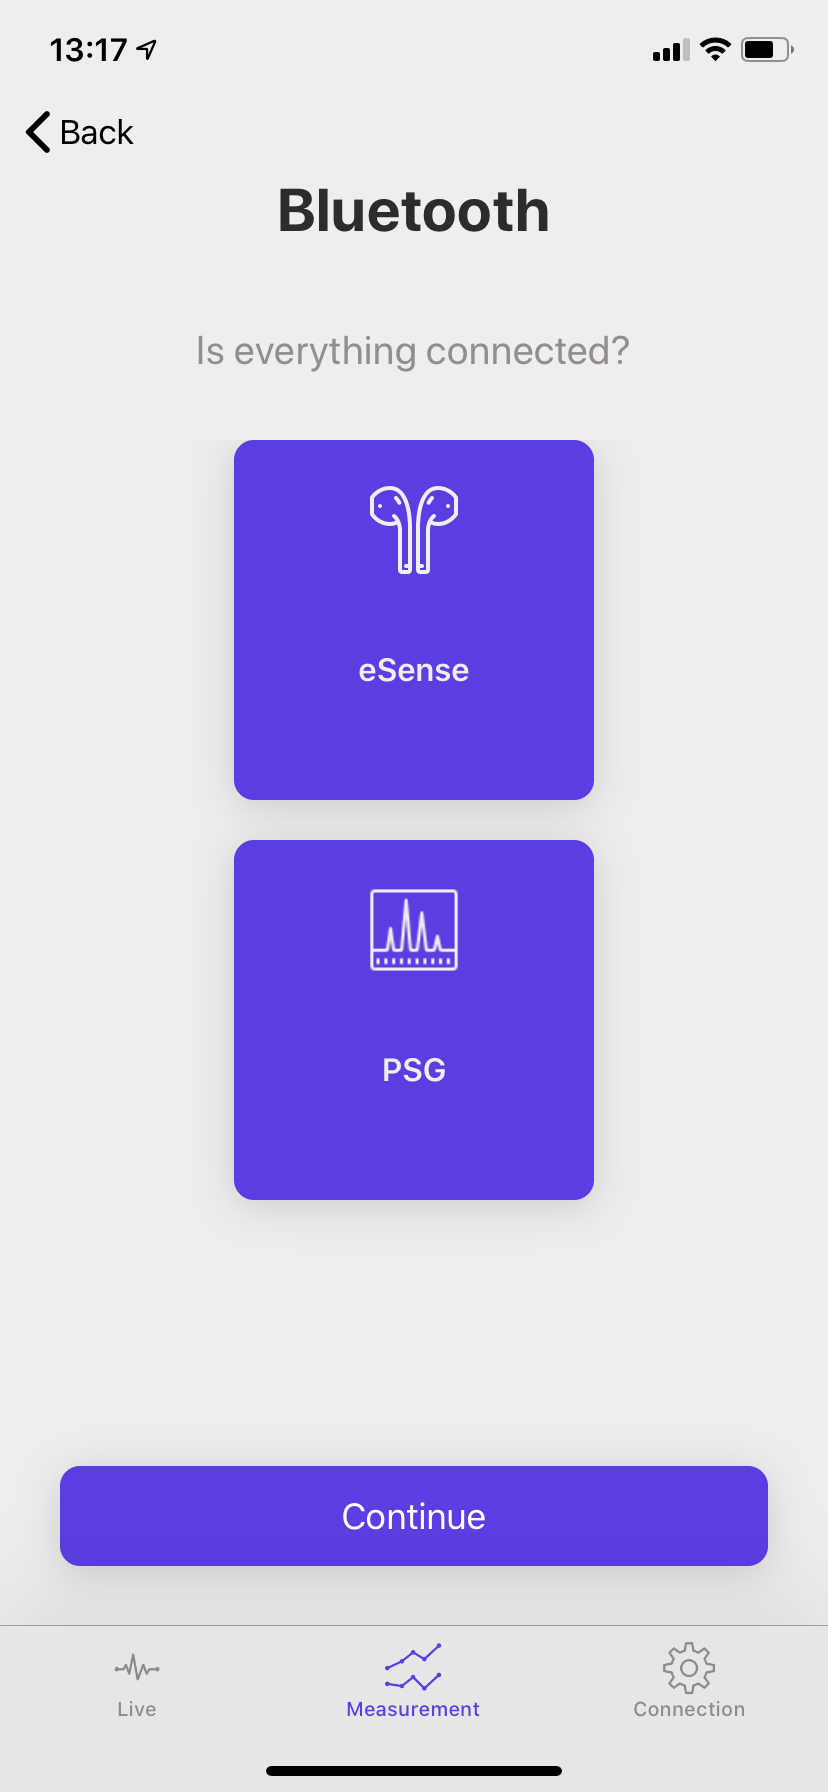
\includegraphics[width=1\textwidth]{app/connect}
    \caption{Verbinden der eSense-Earpods}
    \label{implementation:app:screenshots:connect_bluetooth}
  \end{subfigure}
  \begin{subfigure}{.25\textwidth}
    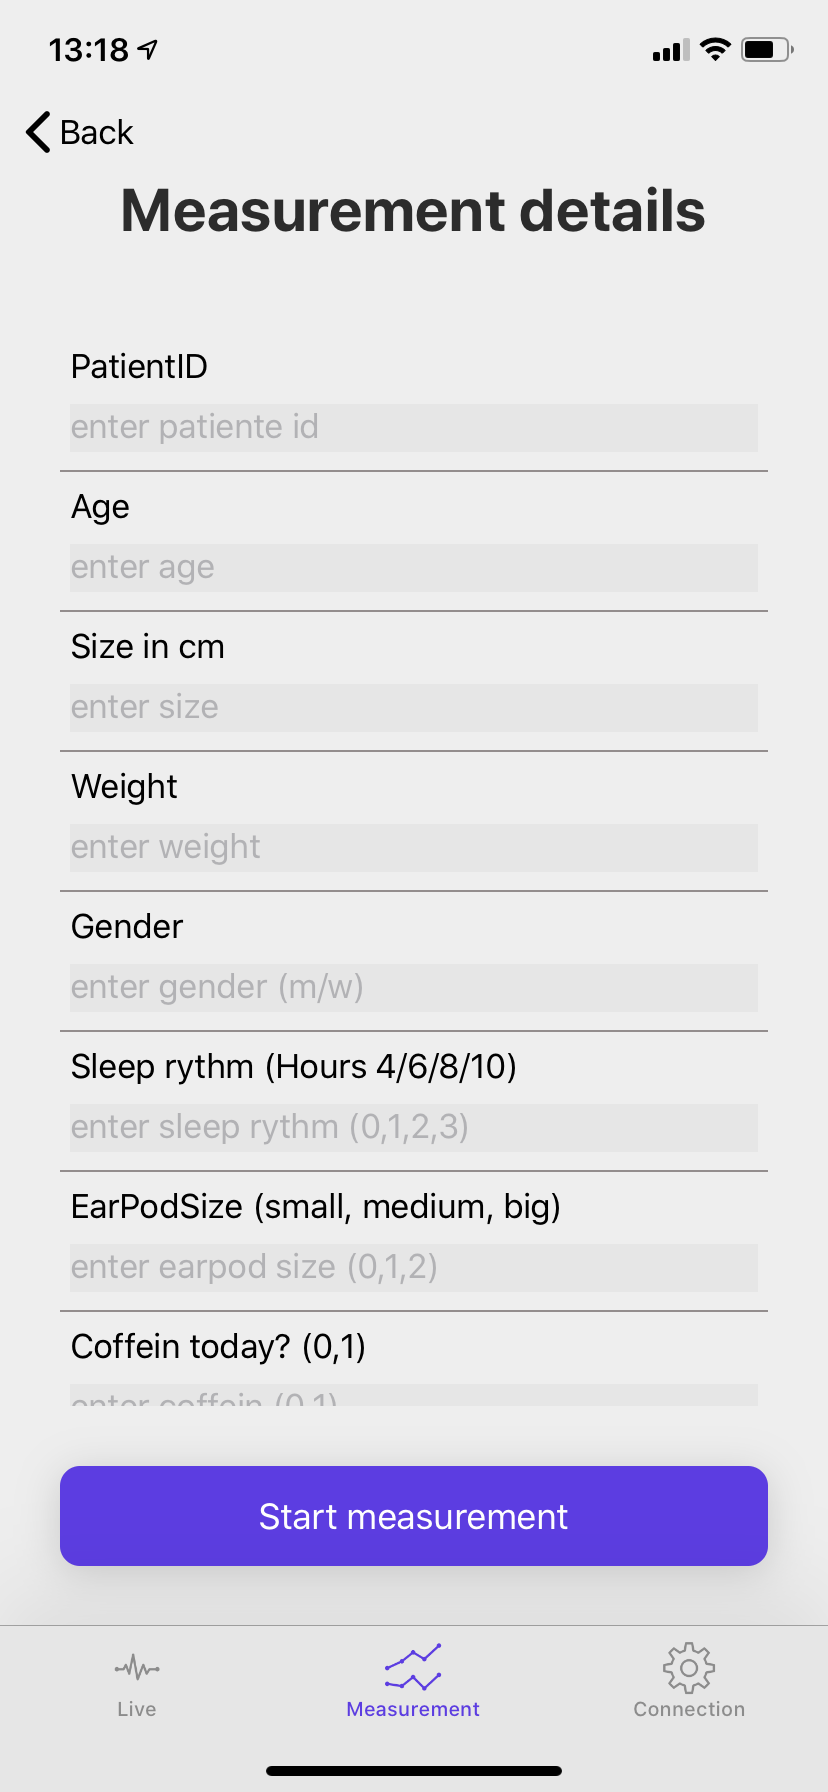
\includegraphics[width=1\textwidth]{app/measurement_details}
    \caption{Eingabe der Nutzerinformationen}
    \label{implementation:app:screenshots:user_studies_information}
  \end{subfigure}
  \begin{subfigure}{.25\textwidth}
    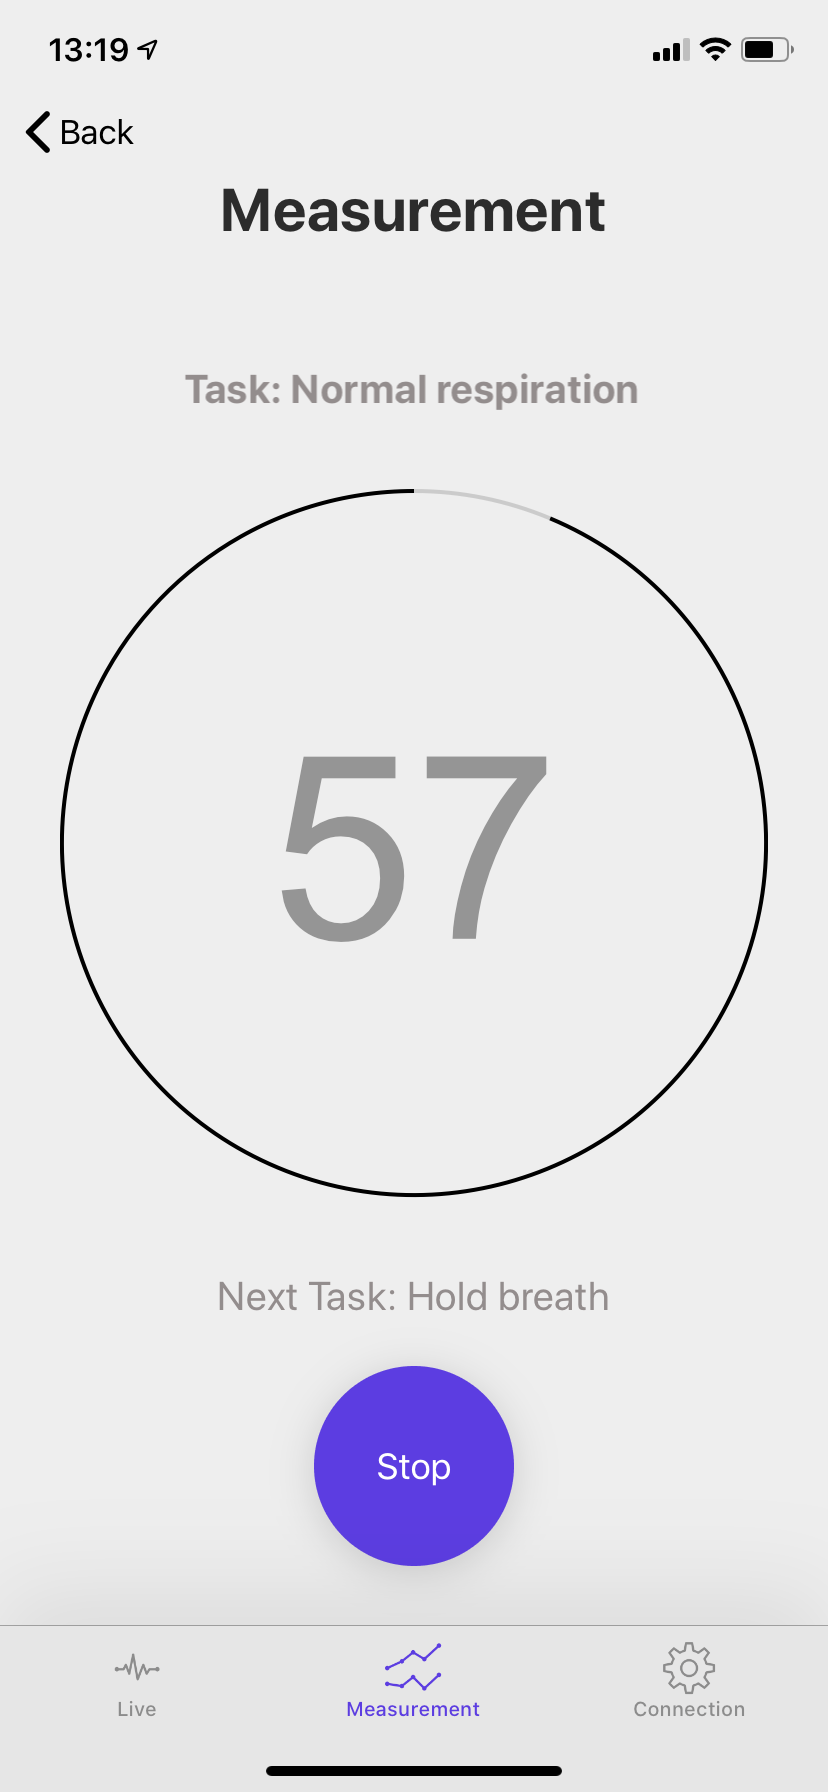
\includegraphics[width=1\textwidth]{app/measurement_timer_02}
    \caption{Messung, aktueller und nächster Task}
    \label{implementation:app:screenshots:measurement_started}
  \end{subfigure}
  \begin{subfigure}{.25\textwidth}
    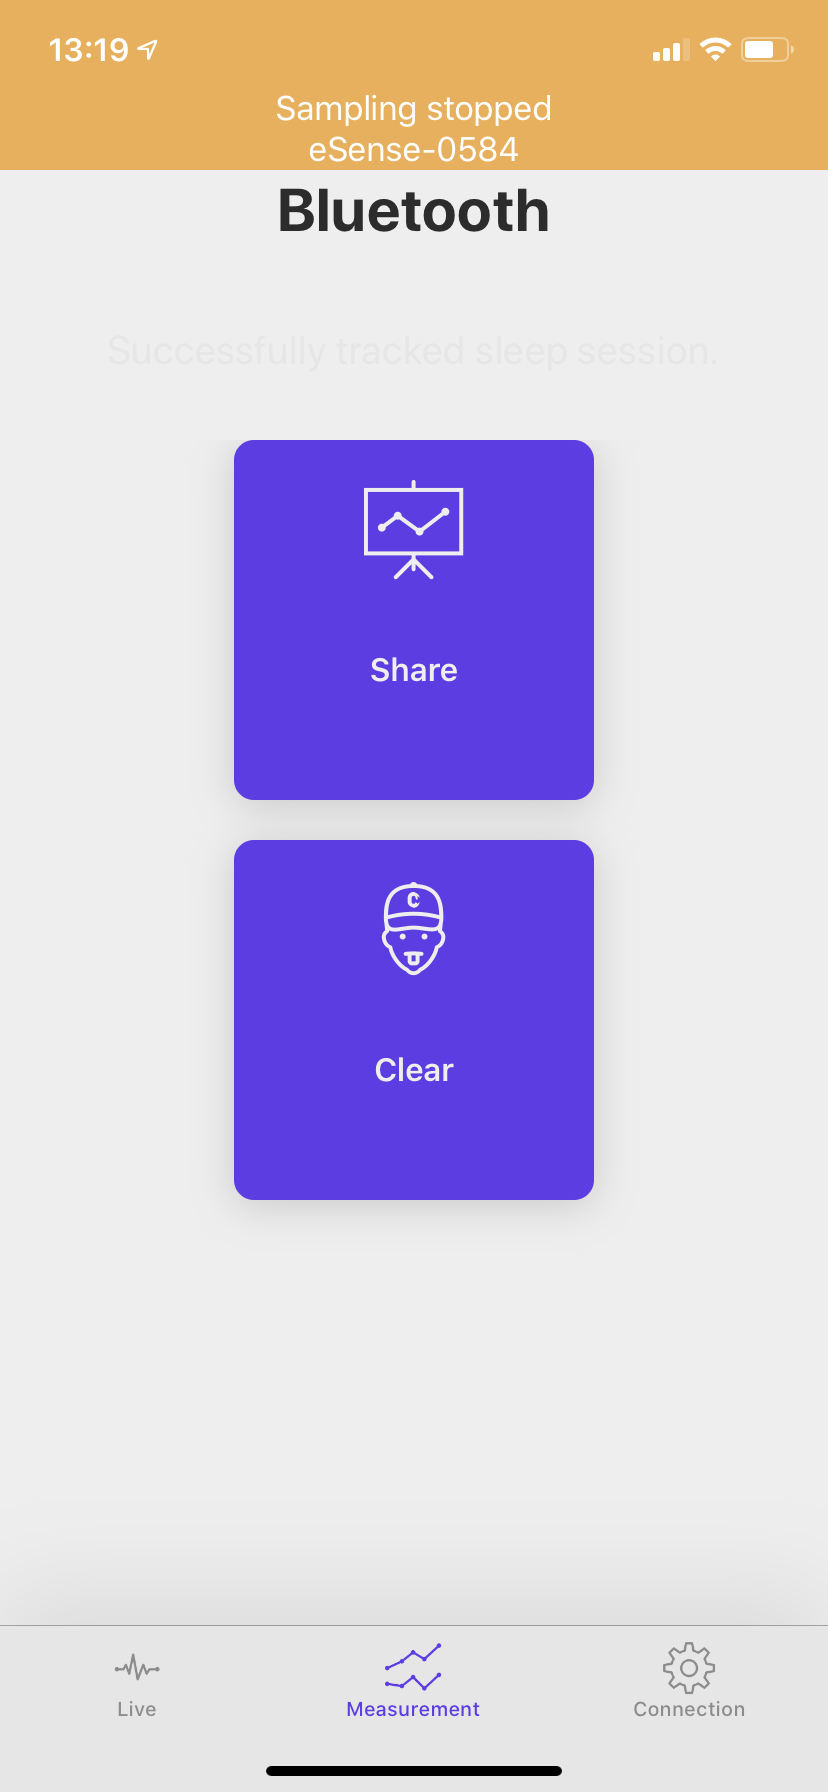
\includegraphics[width=1\textwidth]{app/measurement_finished}
    \caption{Messung beendet}
    \label{implementation:app:screenshots:sampling_stopped}
  \end{subfigure}
  \begin{subfigure}{.25\textwidth}
    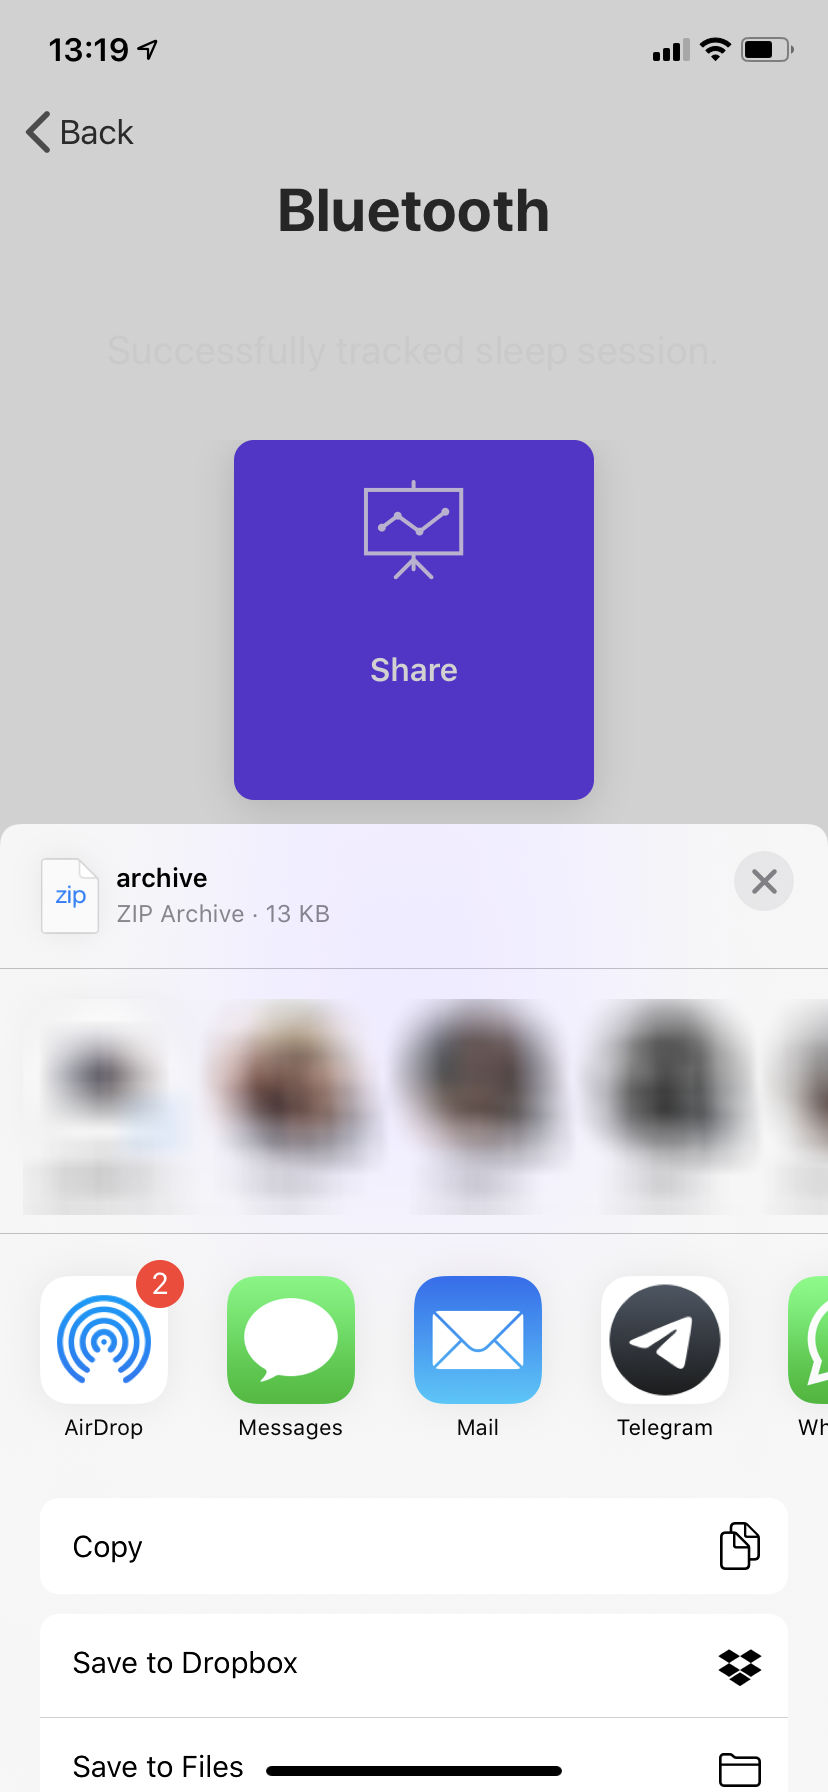
\includegraphics[width=1\textwidth]{app/measurement_share}
    \caption{Messung teilen}
    \label{implementation:app:screenshots:share}
  \end{subfigure}
  \caption{Verlauf einer Messung mit der App}
  \label{implementation:app:screenshots}
\end{figure}

\subsection{Synchronisation der Daten}
\label{ch:Implementierung:data_sync}
Da es nicht garantiert ist, dass der Timer des PSG-Systems zuverlässig arbeitet, wird jeder Peak des Lichtsensors mit dem Lichtsignal der Smartphone-Daten verglichen.
Der Abstand jedes einzelnen Peaks wird nun ermittelt und die durchschnittliche Distanz der Peaks wird ermittelt.
In der Abbildung \ref{implementation:synchronisation:before_light_peak} ist der Vergleich eines Lichtblitzes von Smartphone (blau) und PSG-System (orange) im zeitlichen Verlauf (\texttt{time}).
Da die Verschiebung des Timers des PSG-Systems währrend einer 7-minütigen Messung im Mittel bei $0.3\si{\s}$ lag, wurde der Timer des PSG-Systems um die durchschnittliche Distanz der Peaks verschoben.
Dies ist ausreichend, da die PSG-Daten in der Bachelorarbeit lediglich zum visuellen Vergleich dienen und in der Klassifikation nicht mit betrachtet werden. 
Die zeitliche Verschiebung wird nun in jede \textit{csv}-Datei eingearbeitet mit der Zeile \texttt{new\_time}.
In Abbildung \ref{implementation:synchronisation:after_light_peak} ist klar zu erkennen, dass der neue Zeitwert (\texttt{new\_time}) des PSG-Signals (orange) direkt über dem Zeitwert des Smartphonesignals (blau) liegt, was an den Lichtpeaks zu erkennen ist.
Nun ist garantiert, dass die Lichtsignale von PSG-System und dem Smartphone annähernd synchron sind. Die Daten sind nun bereit zur Analyse.

\begin{figure}[ht]
  \centering
  \begin{subfigure}{0.66\textwidth}
    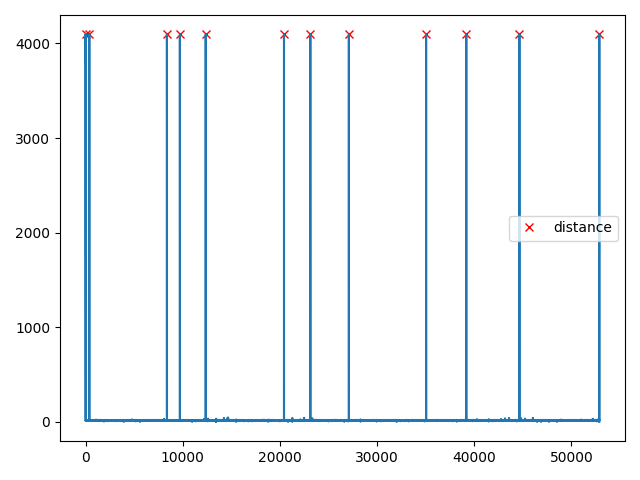
\includegraphics[width=1\textwidth]{data_analyzation/light_peak_detection_psg_data}
    \caption{Peaks des Lichtsignals vom PSG-Gerät. Somit können die PSG-Daten und die Daten, gesammelt von den eSense Earpods zeitlich synchronisiert werden. Der Ablauf der Lichtpeaks ist identisch zum Ablauf der Nutzerstudie (siehe Abb. \ref{fig_study_flow}) \todo{bessere grafik und zudem noch dass man alle peaks von der edf sieht und die doppelten signale erkennt, eventuell breitere grafik}}
    \label{implementation:synchronisation:light_peaks_detection}
  \end{subfigure}
  \begin{subfigure}{.49\textwidth}
    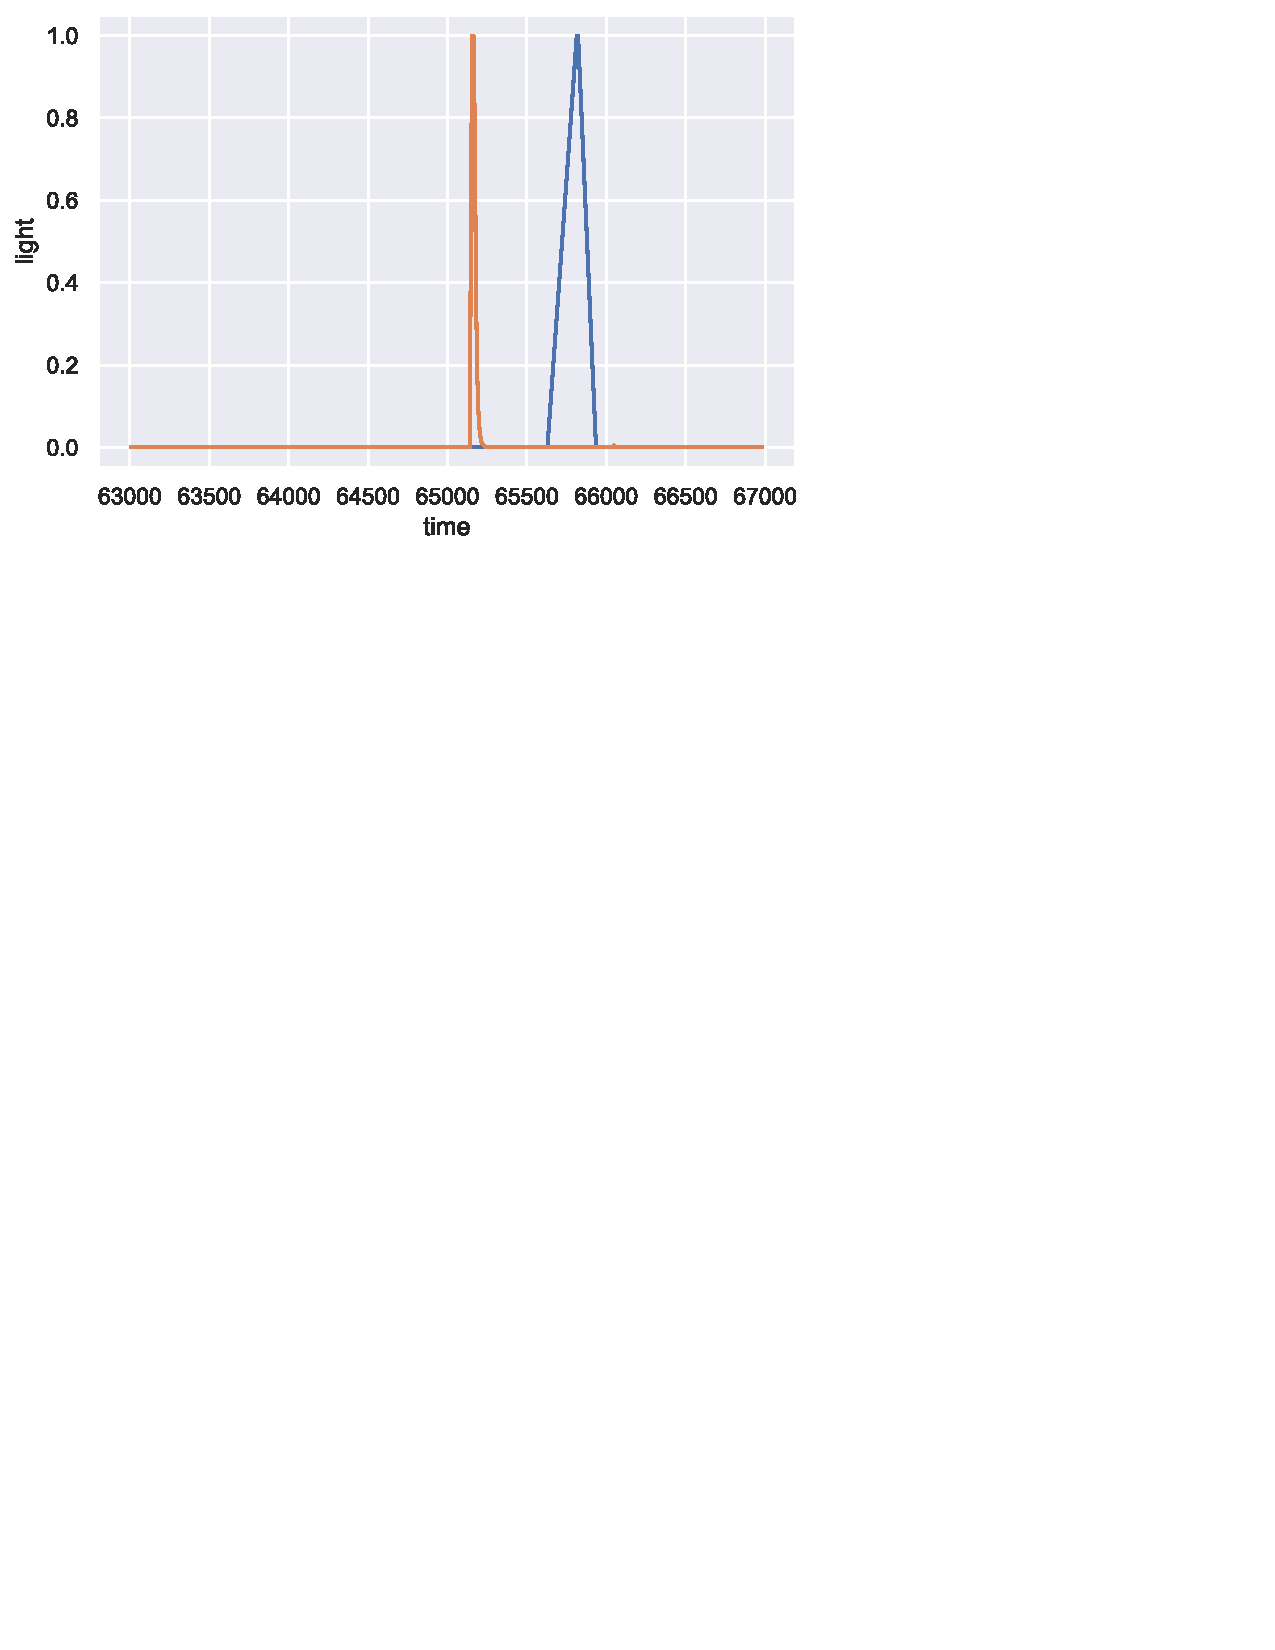
\includegraphics[width=1\textwidth]{data_analyzation/light_peak_detail_before}
    \caption{Zeitlicher Lichtpeakvergleich vor der Synchronisation. Das Lichtsignal des PSG-Geräts (orange) ist weniger als 1s vom Signal der eSense Earpods (blau) entfernt. \todo{modify time value}}
    \label{implementation:synchronisation:before_light_peak}
  \end{subfigure}
  \begin{subfigure}{.49\textwidth}
    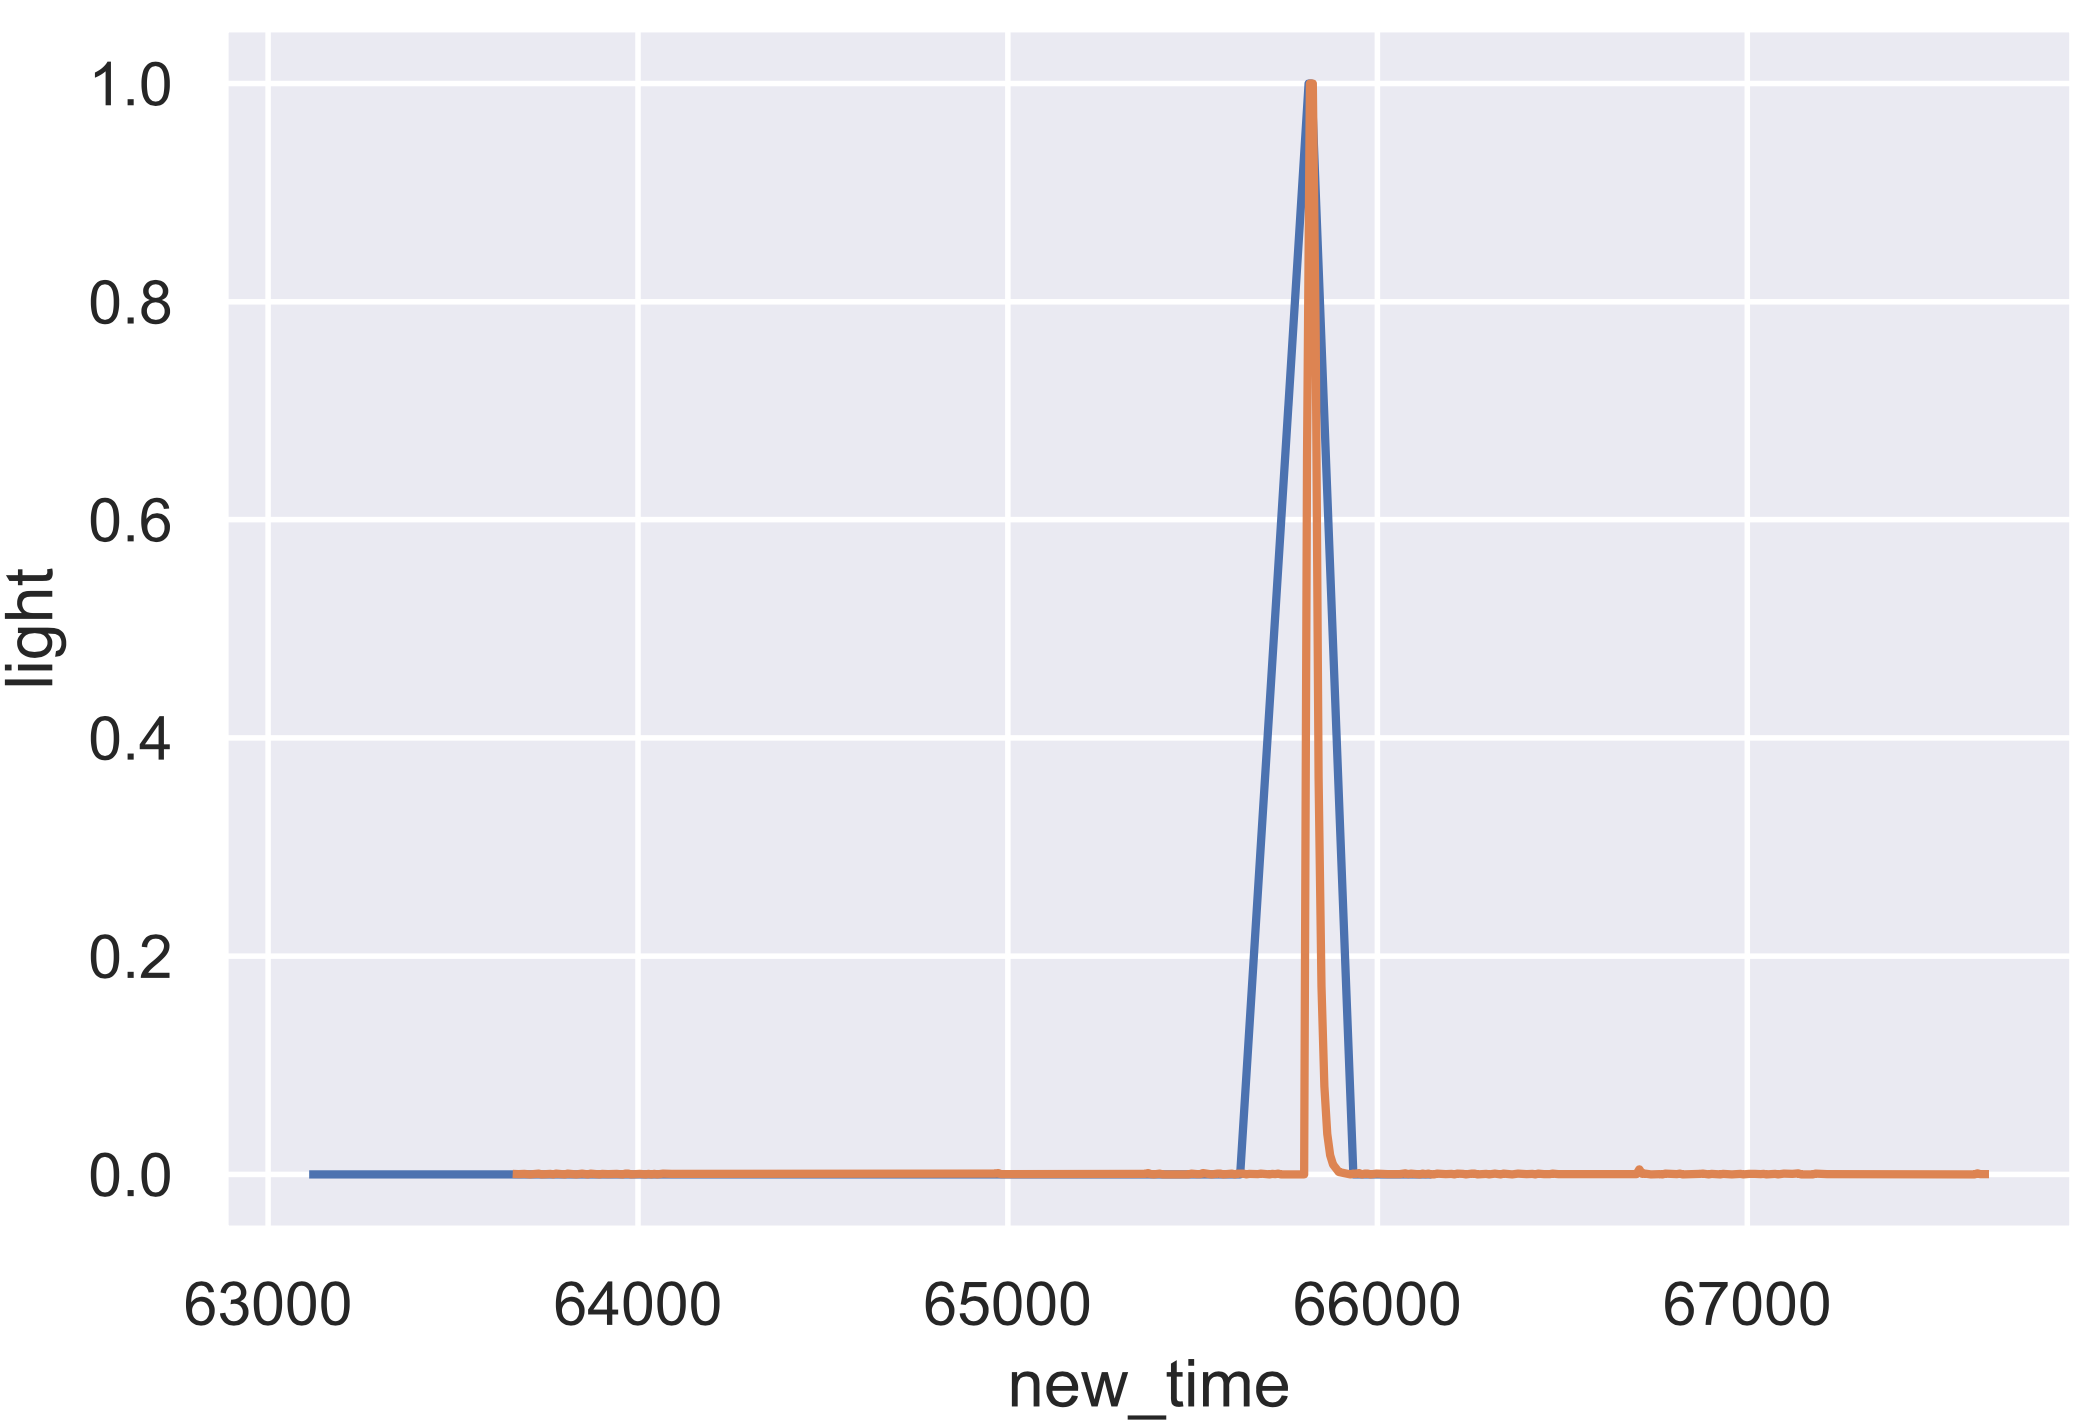
\includegraphics[width=1\textwidth]{data_analyzation/light_peak_detail_after}
    \caption{Zeitlicher Lichtpeakvergleich nach der Synchronisation. Das Lichtsignal des PSG-Systems (orange) ist nun zeitlich sehr nahe über den Lichtpeaks der eSense Earpods (blau)}
    \label{implementation:synchronisation:after_light_peak}
  \end{subfigure}
  \label{implementation:synchronisation}
\end{figure}

\section{Verarbeitungspipeline zur Klassifikation}
\label{ch:Implementierung:classification_pipeline}
Zur Klassifizierung der Daten müssen nun Features berechnet werden. 
Pro Position wurden nun alle Werte in Fenster gepackt mit einer Größe von $5\si{\s}$, beziehungsweise $10\si{\s}$ mit einer Verschiebung von $1\si{\s}$. 
Da die Messergebnisse der eSense Earpods per BLE an das Smartphone gesendet wurden und dort keine Uhrzeit mitgegeben wurde, liegen die einzelnen Messergebnisse nicht im Abstand von exakt $50\si{\hertz}$ vor. 
Aufgrund dessen wurden Fenster manuell anhand des Zeitwertes zusammengefügt. 
Anschließend wurden mittels des Moduls \texttt{tsfresh} Features berechnet und es entstand eine Datei \textit{df\$patient\_id\$\_\$position\_id\$\_feature.csv}.

Da nun die Features für eine Fenstergröße von $5\si{\s}$ und $10\si{\s}$ mit der Verschiebung von $1\si{\s}$ pro Fenster vorliegen, kann mit der Klassifikation begonnen werden.